\begin{frame}{Pre-LayerNorm vs.\ Post-LayerNorm}
  \small
  \begin{table}[ht]
    \centering
    \begin{tabular}{lcc}
      \toprule
      \textbf{Feature} & \textbf{Pre-LN} & \textbf{Post-LN} \\
      \midrule
      Stability & \checkmark\,More stable & \ding{55}\,Less stable \\
      Gradient flow & \checkmark\,Better & \ding{55}\,Can explode/vanish \\
      Used in & GPT-3, T5 & Original Transformer \\
      \bottomrule
    \end{tabular}
    \caption*{\footnotesize\textbf{Table 1:} Comparison of Pre-LayerNorm and Post-LayerNorm Architectures}
  \end{table}

  \vspace{1em}

  \textbf{Pre-LN:} LayerNorm applied \textbf{before} sublayers

  \textbf{Post-LN:} LayerNorm applied \textbf{after} sublayers
\end{frame}

\begin{frame}{Pre-LayerNorm vs.\ Post-LayerNorm}
  \centering
  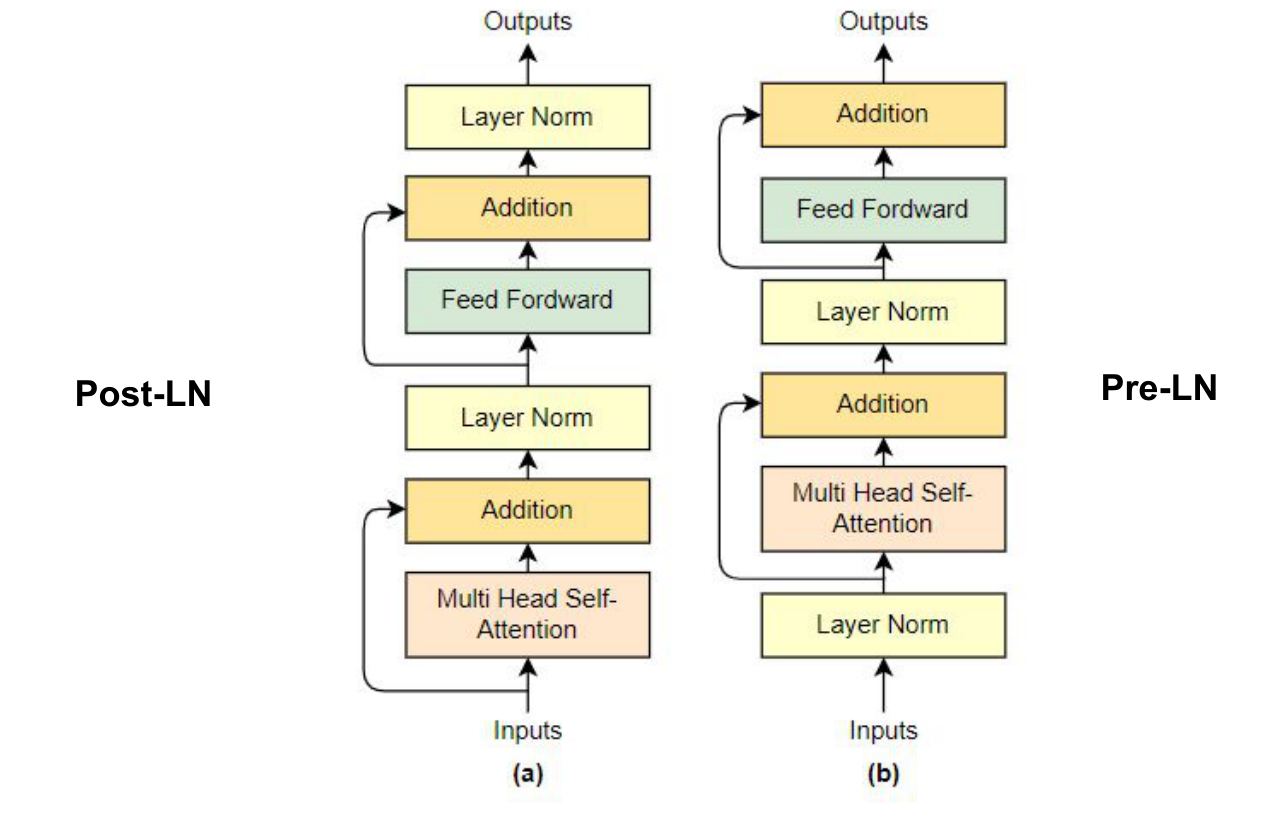
\includegraphics[width=0.8\paperwidth,height=0.8\paperheight,keepaspectratio]{assets/Lecture-6_Introduction_to_Transformers/pdf_page_084.png}
\end{frame}

\begin{frame}{Pre-LayerNorm vs.\ Post-LayerNorm}
  \centering
  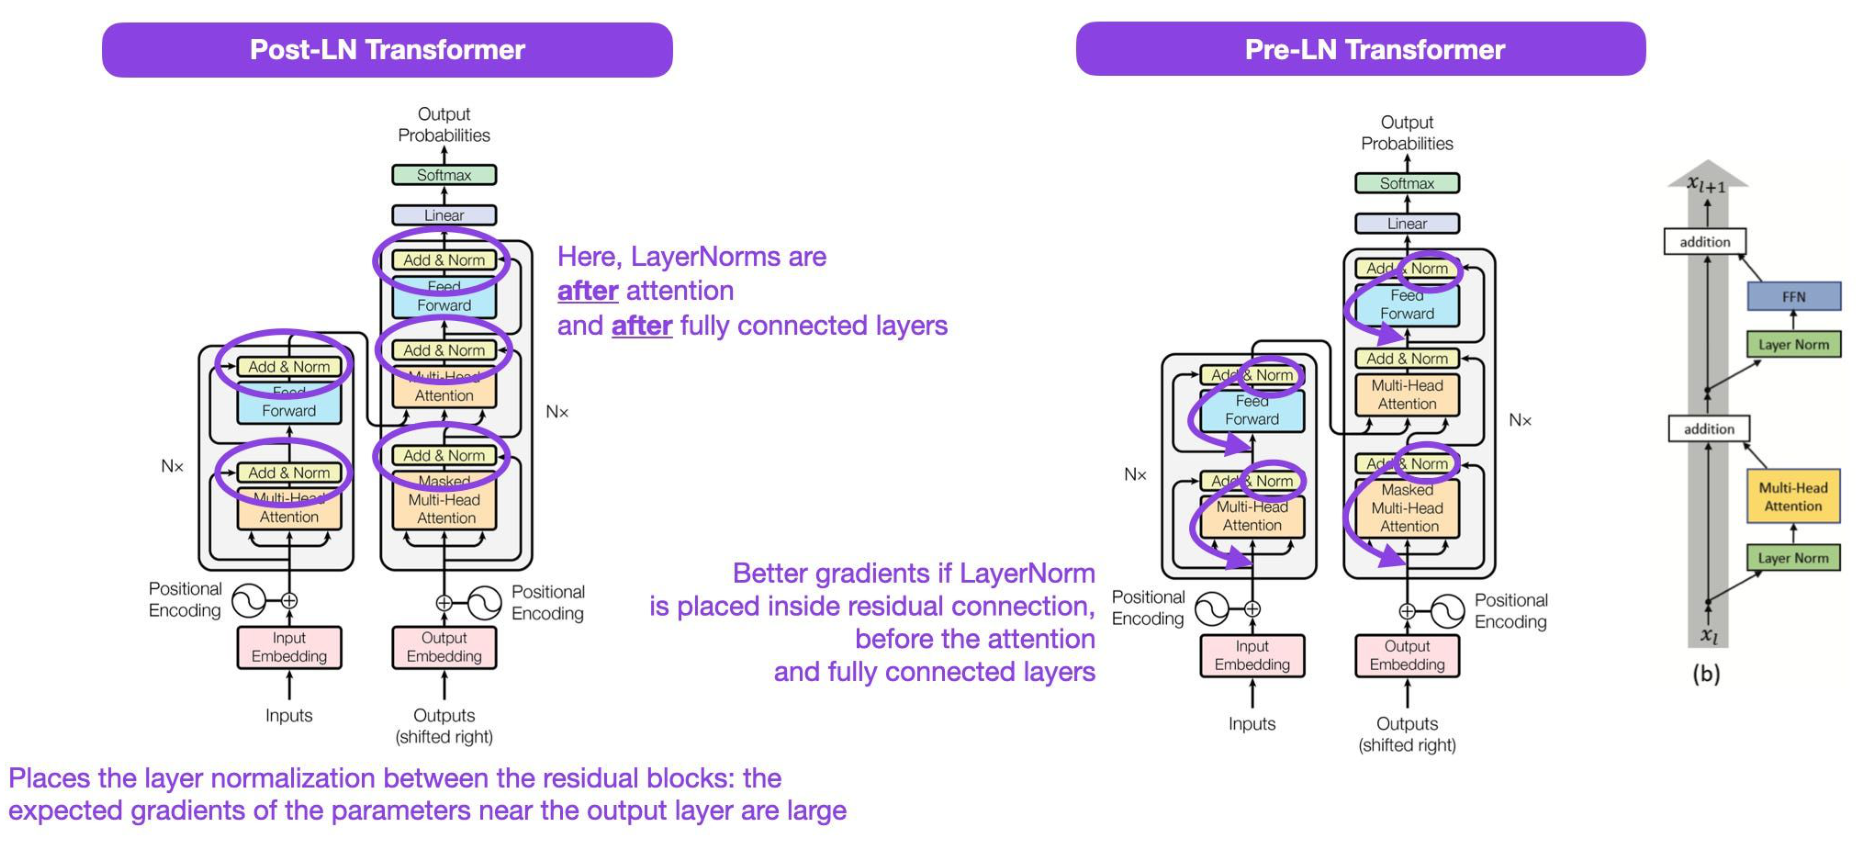
\includegraphics[width=0.9\paperwidth,height=0.9\paperheight,keepaspectratio]{assets/Lecture-6_Introduction_to_Transformers/pdf_page_085.png}
\end{frame} 

\begin{frame}{Pre-LayerNorm vs.\ Post-LayerNorm}
  \centering
    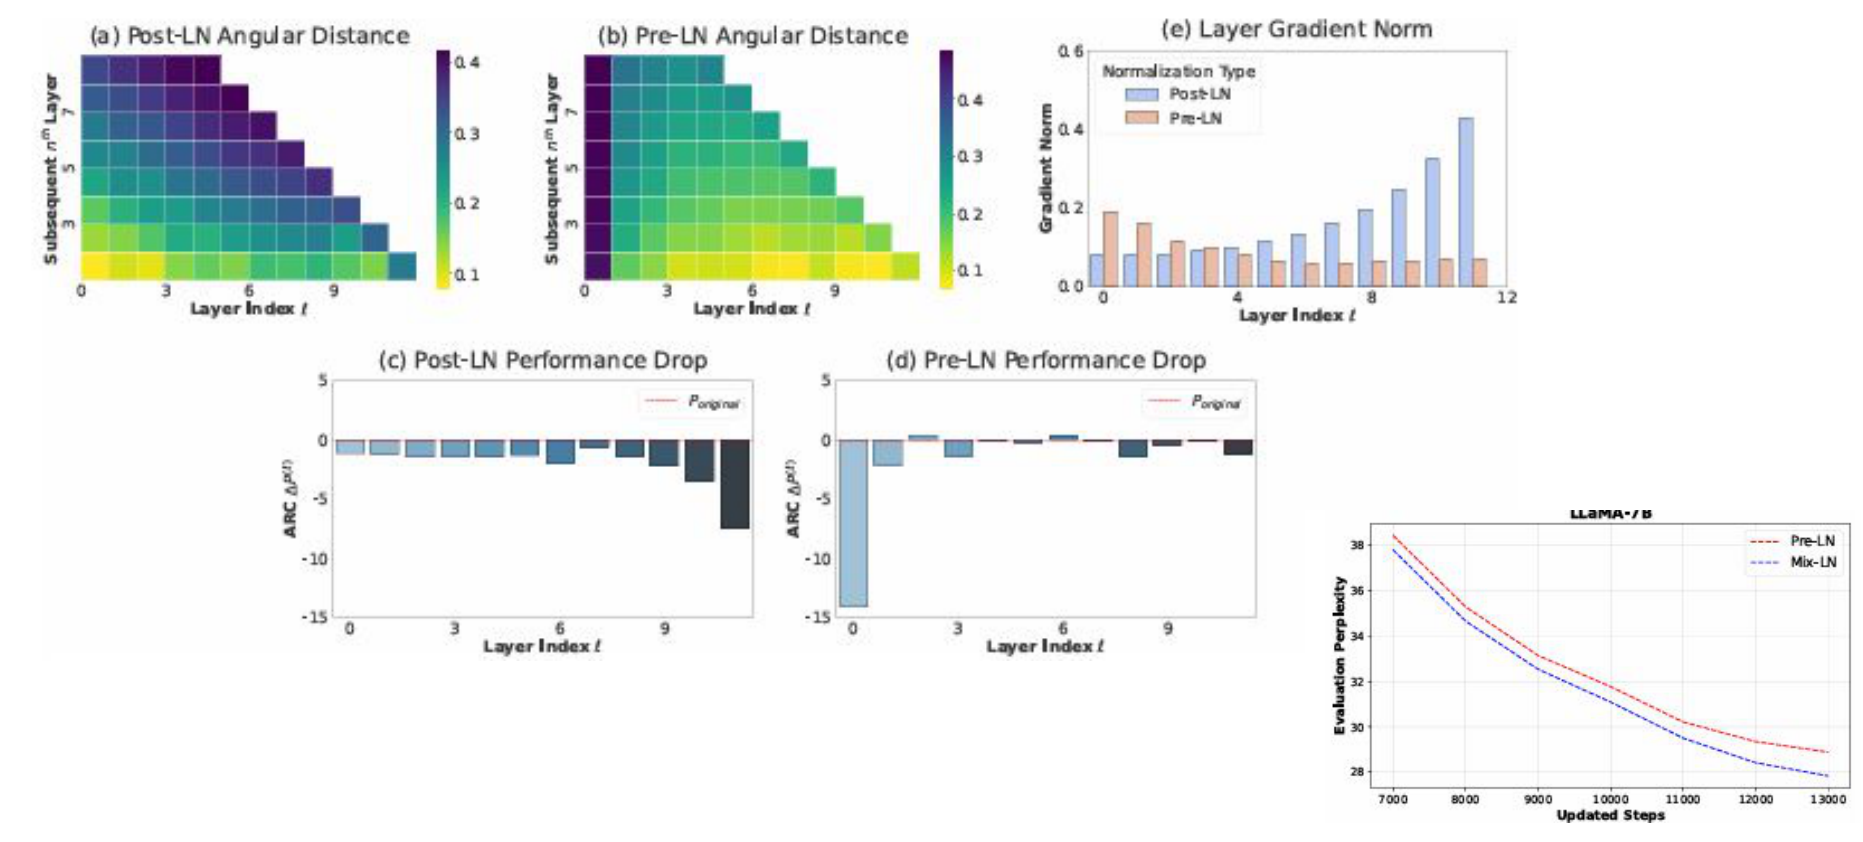
\includegraphics[width=0.9\paperwidth,height=0.9\paperheight,keepaspectratio]{assets/Lecture-6_Introduction_to_Transformers/pdf_page_086.png}
\end{frame}

